\scanpage{67}
\deleted{\unsure{Ainsi}}
\deleted{On sait que}
\deleted{On sait que}

On a d'autre part, si
\[
\deleted{0\longrightarrow\Gamma\longrightarrow}\qquad \unsure{j|j_0}:\Gamma\longrightarrow\operatorname{Pic}(X_0)\qquad\deleted{\unsure{\longrightarrow}}
\]
est le composé, d'où des $j_n:\Gamma_n\mathbin{-}\operatorname{Pic}(X_0)_n$, \deleted{\unsure{on a}} l'inclusion évidente :
\[
\operatorname{Ker}i_n\subset\operatorname{Ker}j_n.
\]
\margin{\uline{Lemme}. $\operatorname{Pic}(X)_n\longrightarrow\operatorname{Pic}(X_0)_n$ (du moins si $S$ complet, ce qui suffit pour le th.) \unsure{faisable par les th. clés}.}
Cette inclusion est \inserted{en fait} une \uline{identité}. Pour le voir, on note que si $L$ est un faisceau inv. sur $X$, et si $L_0=L|X_0$ est écrit comme puissance $n$ième, alors l'obstruction à écrire $L$ lui-même puissance $n$ième est nulle (cf \unsure{FGA|SGA}, exposé sur Picard). On a d'autre part
\[
\operatorname{Pic}(X_0)=\underline{\operatorname{Pic}}_{X_0/k}(k)
\]
\unsure{grâce} au fait que $X_0$ a un cycle de degré 1, d'où
\diagram{\begin{tikzcd}[column sep=large]
0\arrow[r,dash]&\operatorname{Pic}^{0}(X_0)\arrow[r,dash]\arrow[d,equal,"\mathrm{dfn}"']&\operatorname{Pic}(X_0)\arrow[r]&\operatorname{NS}(X_0)'\arrow[r]\arrow[d,equal,"\mathrm{dfn}"']&0\\
&\underline{\operatorname{Pic}}^{0}_{X_0/k}(k)&&\operatorname{Im}\bigl(\underline{\operatorname{Pic}}_{X_0/k}(k)\longrightarrow\underline{\operatorname{NS}}_{X_0/k}(k)\bigr)
\end{tikzcd}}
et $\operatorname{Pic}^{0}(X_0)$ est $n$-divisible, donc on a
\[
\operatorname{Pic}(X_0)_n\longrightarrow\operatorname{NS}(X_0)_n.
\]
\margin{\unsure{joindre au lemme précédent}}
donc si
\[
\unsure{k}:\Gamma\mathbin{-}\operatorname{NS}(X_0)
\]
est le composé $\Gamma\xrightarrow{j}\operatorname{Pic}(X_0)\longrightarrow\operatorname{NS}(X_0)$, on trouve
\[
\operatorname{Coker}u_n\simeq\operatorname{Ker}\unsure{k_n}.
\]
Je dis que \inserted{$\Gamma$ est sans torsion et que} $\unsure{k|\delta}$ est \uline{injectif}, i.e. qu'un faisceau inv. sur $X$ qui est trivial sur $X_\eta$, et qui sur $X_0$ est \deleted{\unsure{num.}} équiv. à zéro, est trivial.
\margin{cf plus bas une démonstration}
\inserted{$\unsure{L^l\simeq\mathcal O}\ \unsure{par l'imp.}$}
\deleted{\unsure{dans} $\operatorname{NS}(X_0)$ est nulle \unsure{implique par le critère (ou négativité) que} \unsure{pour ce est impossible le diviseur} \unsure{par} $\unsure{l\ne p}$, \unsure{et il peut faire le diviseur de} \unsure{fibre générique, en prenant dans} \unsure{Hensélisé un trait, on trouvera}}
\figure{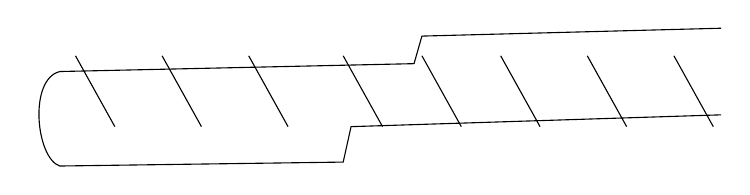
\begin{tikzpicture}[x=1cm,y=1cm]
\draw (0,1.4)--(4.5,1.5)--(4.6,1.85)--(8.4,1.95);\draw (0,1.4) .. controls (-.4,1.3) and (-.3,.3) .. (0,.2)--(3.6,.25)--(3.7,.7)--(8.4,.85);
\foreach \x in {.2,1.3,2.4,3.6,4.6,5.6,6.7,7.8}{\draw (\x,1.6)--(\x+.5,.7);}
\end{tikzpicture}}
une suite exacte
\deleted{\diagram{\begin{tikzcd}
0\arrow[r,dash]&\Gamma\arrow[r,"\unsure{k}",dash]&\operatorname{NS}(X_0)'\arrow[r,dash]&\unsure{\delta}\arrow[r]&0
\end{tikzcd}}}
\deleted{$\unsure{\operatorname{Coker}k=\operatorname{Coker}\Delta}$}
\deleted{$\unsure{\operatorname{Coker}\Delta}$}
\inserted{\diagram{\begin{tikzcd}[column sep=small]
0\arrow[r]&\Gamma\arrow[r,"k'"]&\operatorname{NS}(X_0)'\arrow[r,"\lambda"]\arrow[d,equal]&\delta\arrow[r]&0\\
&&\text{\unsure{sous-groupe de} }\operatorname{NS}(X_0)\text{ \unsure{dont un multiple donne dans} }\Gamma
\end{tikzcd}}}
d'où par le \unsure{sens} habituel
\[
\deleted{\unsure{donc}}\quad \operatorname{Ker}k_n=\operatorname{Ker}k'_n\simeq\operatorname{Coker}{}_n\lambda.
\]
Comme $\Gamma$ est sans torsion, \deleted{\unsure{on}} $\delta'\xrightarrow{\lambda}\delta$ est injectif, et on trouve que $\operatorname{Coker}{}_n\lambda={}_n\delta/{}_n\delta'$. On termine grâce à la suite
\margin{66}
